\chapter{Fundamentals and Related Work\label{cha:relatedwork}}

This chapter is intended to give an introduction about relevant terms, technologies and
standards in the field of Deep Learning and Generative Adversarial Networks. It also
covers some necessary backgrounds to get the basic overview of the topic.

\section{Classification using Deep Learning}
As we already mentioned in Chapter \ref{cha:introduction}, \acrfull{dl} is a powerful
\acrshort{ml} tool. It has a lot of advantages comparing to the other traditional methods.
In many cases, it does not need a thorough and careful Feature Extraction, and the
multiple-layer nature enable it to learn multiple levels of features from the data. In
this section, the author would like to discuss some relevant backgrounds on \acrshort{dl}
and how people use it for Object Classification.

Classification is a basic task in \acrshort{ml}, and Image Classification has become a
very common application of Deep Learning since the beginning because of the potential
applications, availability of data, and the pixel structure of the images in which every
pixel can be assumed to be independent from the other. The last point is a very important
assumption in a lot of \acrshort{ml} applications. 

Because of the popularity of the topic, a lot of researchers have been spending efforts on
designing and training different architectures to get the best results.  Different works
are usually evaluated on some standard labeled datasets. The accuracies on those datasets
are considered as the performance metric of a network. ImageNet \todo{cite ImageNet} is
one of the biggest and most popular Object Image Database available, consisting of
millions of images. On ImageNet, Krizhevsky et al. \todo{cite AlexNet} trained an 8-layer
Convolutional Neural Networks which achieved significantly lower error rates than the
State-Of-The-Art methods at the publication time.

\subsection{Transfer Learning}
If we take a closer look at a Deep Classification Network such as AlexNet \todo{cite
AlexNet}, we can see that the last layer is often a Softmax layer, which does nothing more
than converting the output to the range $[0, 1]$ so that we have a prediction probability
of each class. The real classification work is done in the previous layer (fc8), where the
probability that the object image belongs to each class is calculated by a Linear
Regression. In AlexNet, as we have 1000 classes, we have 1000 neurons in fc8 corresponding
to 1000 Linear Regressions. The intuition here is that, the input of that decision layer
should be a good representation of the data if the network is performing well. In
principle, we can reuse the output of the layer before fc8, which is fc7, in other
\acrshort{ml} tasks. That forms the basic idea of Transfer Learning.

\subsection{AlexNet}
As mentioned above, AlexNet is one of the classical approaches of using Deep Neural
Network to solve the Object Classification task on the huge dataset ImageNet.  AlexNet
consists of 8 layers as shown in Figure~\ref{fig:alexnet}. There are 5 convolutional
layers and 3 fully-connected layers. The last layer is connected to a 1000-way Softmax
layer because the ImageNet dataset \todo{cite ImageNet} used to train the network contains
1000 classes.

\begin{figure}[htb]
  \centering
  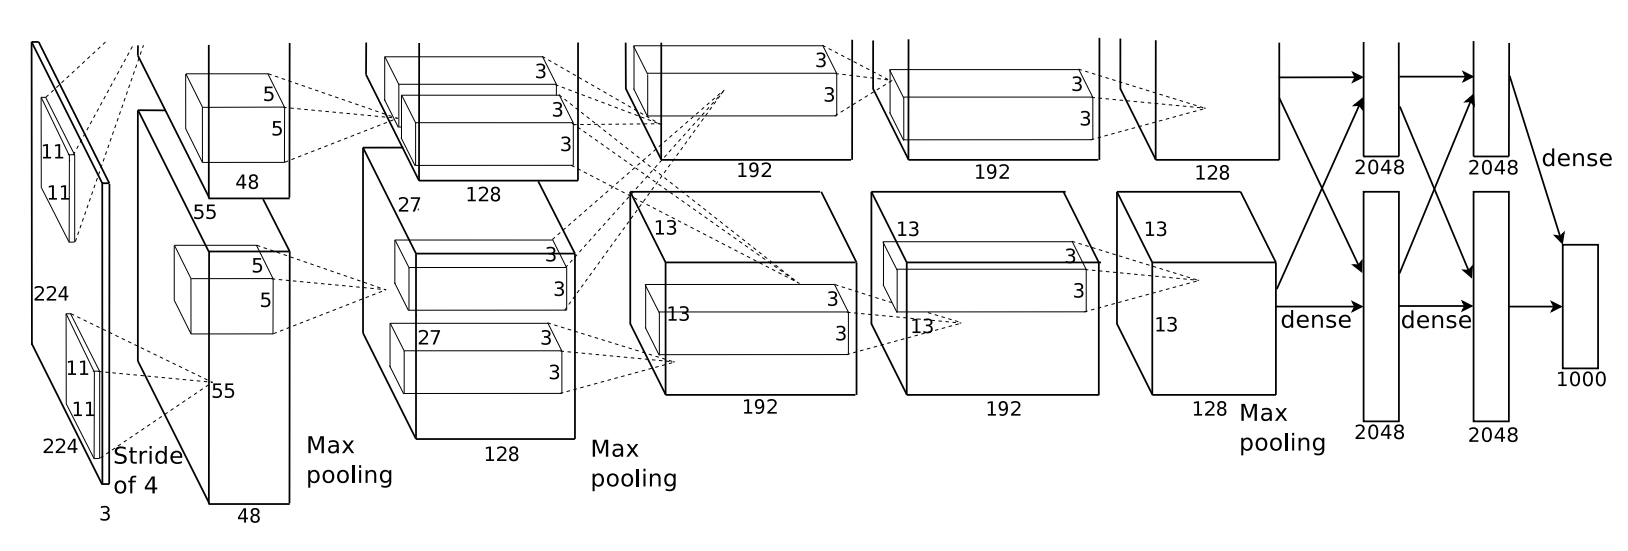
\includegraphics[width=0.9\textwidth]{alexnet_architecture}
  \caption{AlexNet Architecture}\label{fig:alexnet}
\end{figure}

\subsection{Object Recognition on Washington RGB-D dataset \todo{cite eitel et al}}
Transfer Learning is the main idea of Eitel et al. \todo{cite Eitel}. In the paper, the
authors use an implementation of AlexNet in Caffe (CaffeNet) to get the representations of
the objects in the Washington RGB-D dataset. The representations are then fed into a
fully-connected layers where the final results are connected to a 51-way Softmax layers to
classify 51 different classes in the Washington Object Dataset \todo{cite Washington}.
Figure \ref{fig:eitel_net} describes the network.

\begin{figure}[htb]
  \centering
  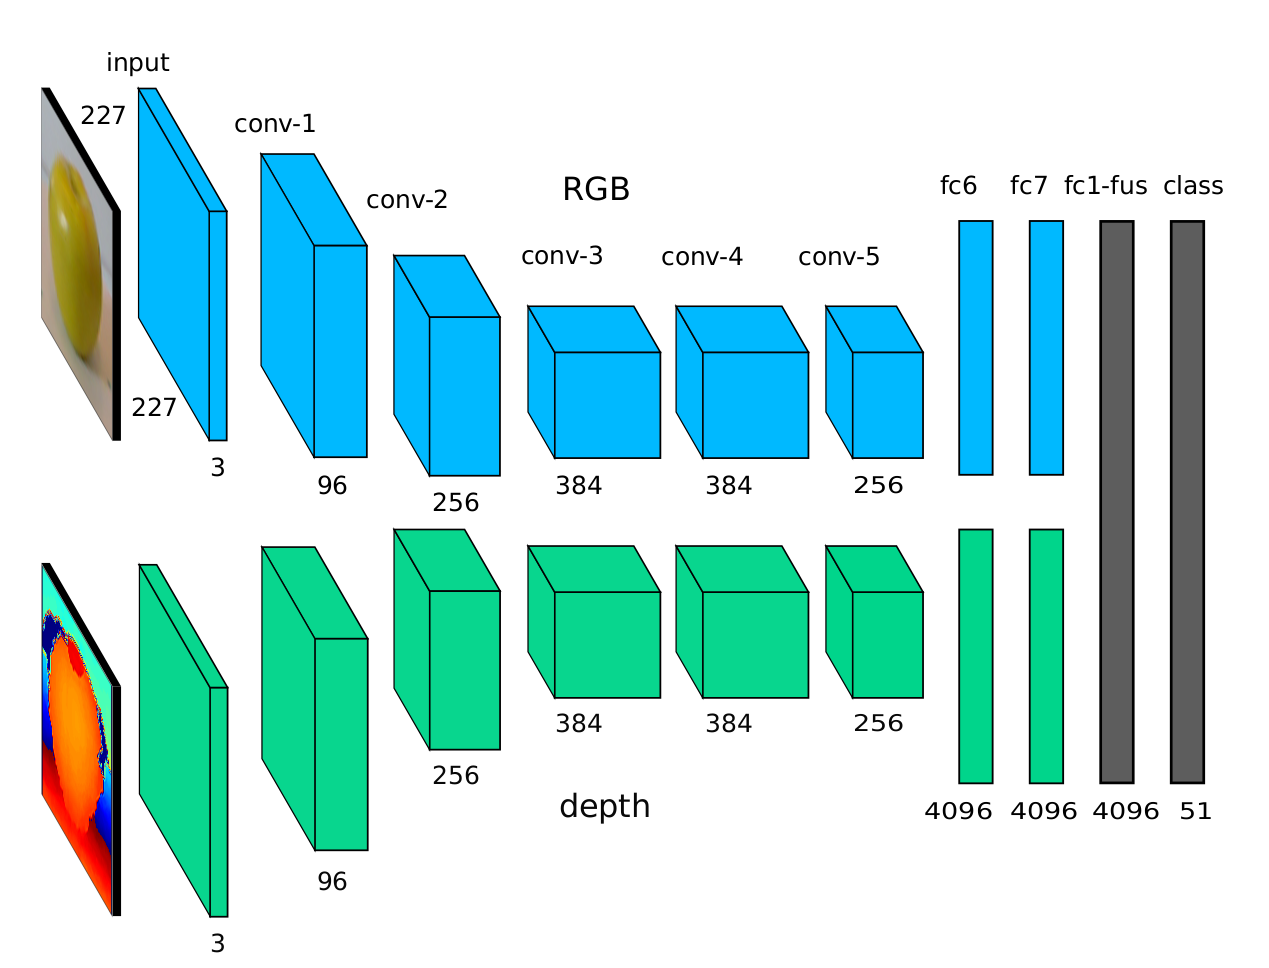
\includegraphics[width=0.9\textwidth]{eitel_net}
  \caption{Eitel et al. architecture for Object Classification}\label{fig:eitel_net}
\end{figure}

\section{Generative Adversarial Networks}
\section{Pix2pix}

